\documentclass[a4paper, 14pt]{extarticle}


% ====== Localization & fonts ======
\usepackage{xcolor}
\usepackage{fontspec}
\usepackage{polyglossia} % Russian lang
\setdefaultlanguage{russian}
\setmainfont{Times New Roman}[Mapping=tex-text]
\newfontfamily\cyrillicfont{Times New Roman}[Mapping=tex-text]

% TODO look for better; don't like this one
\setmonofont[Scale=0.9]{DejaVu Sans Mono}
\newfontfamily{\cyrillicfonttt}{DejaVu Sans Mono}[Scale=0.8]

% ====== Math ======
\usepackage{amsmath} % Math stuff
\usepackage{gensymb}
\usepackage{amssymb}

% ====== Other text spacing ======

\usepackage{setspace} % String spacing
\onehalfspacing{}

\usepackage{parskip} % The red line
\setlength{\parskip}{15pt} % Sep beetween paragraphs

\usepackage{enumitem}
\setlist{nosep, topsep=-10pt} % Remove sep-s beetween list elements

% ====== Source code listings ======

\usepackage{listings} % Source code
\lstset{
    basicstyle=\ttfamily,
    breaklines=true,
    breakatwhitespace=true,
    commentstyle=\color{green},
    keywordstyle=\bfseries\color{blue},
    tabsize=4
}

\lstdefinestyle{num}{
    numbers=left,
    numbersep=0.5cm,
    numberstyle=\ttfamily,
    xleftmargin=0.85cm,
}

\lstdefinestyle{framed_num}{
    frame=single,
    numbers=left,
    numbersep=0.5cm,
    numberstyle=\ttfamily\color{red},
    xleftmargin=1cm,
    framexleftmargin=1cm
}

\lstdefinestyle{sql_style}{
    morekeywords=[10]{while, do, procedure, begin, end, if, tinyint, enum, datetime, boolean, declare, function, return, deterministic, is}
}

\renewcommand{\lstlistingname}{Листинг}

% ====== CSV ======
\usepackage{csvsimple} % Load CSV

% ====== References ======
\usepackage{hyperref} % Links
\hypersetup{
    colorlinks,
    citecolor=black,
    filecolor=black,
    linkcolor=black,
    urlcolor=black
}


% ====== Captions ======
\usepackage{caption}
\usepackage{subcaption}
\captionsetup[figure]{name=Рисунок, labelsep=endash, parskip=0pt}

\captionsetup[lstlisting]{
    labelsep=period,
    justification=RaggedLeft,
    parskip=0pt,
    singlelinecheck=false,
    skip=3pt
}

\captionsetup[table]{
    labelsep=period,
    justification=RaggedLeft,
    parskip=0pt,
    singlelinecheck=false,
    skip=3pt
}

\captionsetup[figure]{
    name=Рисунок,
    justification=centering,
    labelsep=period,
    parskip=6pt,
    skip=3pt
}

% ====== Misc ======
\usepackage{metalogo} % Logos for LaTeX
\usepackage{lipsum} % Lorem ipsum
\usepackage{graphicx} % Pictures
\usepackage{tabularx} % X-tables
\usepackage{csquotes} % French quoutes
\usepackage{multirow}

\usepackage{lastpage}

\usepackage{placeins} % FloatBarrier

\usepackage[final]{pdfpages} % Include PDF
\setboolean{@twoside}{false}

% ====== Plotting ======
\usepackage{tikz}
\usepackage{pgfplots}
\usepackage{pgfplotstable}
\pgfplotsset{compat=newest}
\usepgfplotslibrary{dateplot}


% ====== My commands ======
\newcommand{\addonsubheader}[1]{{\center{\bfseries \vspace{-0.5cm} #1} \\ \vspace{15pt}}}

\newcommand{\screenshot}[3]{
    \begin{figure}[h]
        \centering
        \includegraphics[#1]{#2}
        \caption{#3}
    \end{figure}
}

% ====== Counters ======

\numberwithin{equation}{section}

\newcounter{stepcounter}[subsubsection]

\newcommand\steppar[2][\DefaultOpt]{
    \def\DefaultOpt{#1}
    \refstepcounter{stepcounter}
    \paragraph{{#2}.\thestepcounter.}
}

% ====== Document sectioning ======
\usepackage{titlesec}
\titleformat*{\section}{\bfseries}
\titleformat*{\subsection}{\bfseries}
\titleformat*{\subsubsection}{\bfseries}
\titleformat*{\paragraph}{\bfseries}
\titleformat*{\subparagraph}{\bfseries\itshape}% chktex 6

\titlespacing*{\section}{0pt}{12pt}{3pt}
\titlespacing*{\subsection}{0pt}{6pt}{3pt}
\titlespacing*{\subsubsection}{0pt}{6pt}{0pt}
\titlespacing*{\paragraph}{0pt}{6pt}{6pt}
\titlespacing*{\subparagraph}{0pt}{6pt}{3pt}

% ====== Page layout ======
\usepackage[ % Margins
left=3cm,
right=2cm,
top=2cm,
bottom=2cm	
]{geometry}

\begin{document}
\begin{titlepage}
    \centering
    {\bfseries
        \uppercase{
            Минобрнауки России \\
            Санкт-Петербургский государственный \\
            Электротехнический университет \\
            \enquote{ЛЭТИ} им. В.И.Ульянова (Ленина)\\
        }
        Кафедра МО ЭВМ

        \vspace{\fill}
        \uppercase{Лабораторная работа №1} \\
        по дисциплине \enquote{Криптография и защита информации} \\
        Тема: Изучение классических шифров средствами RailFence, Scytale, Caesar
    }

    \vspace{\fill}
    \begin{tabularx}{0.8\textwidth}{l X c r}
        Студент гр. 6304 & & \underline{\hspace{3cm}} & Корытов П.В.\\
        Преподаватель & & \underline{\hspace{3cm}} & Племянников
    \end{tabularx}

    \vspace{1cm}
    Санкт-Петербург \\
    \the\year{}
\end{titlepage}

\newpage

\section*{Цель работы}
Исследовать шифры Rail Fence, Scytale, Caesar и получить практические навыки работы с ними, в том числе и в программногом продукте Cryptool 1 и 2.

\section*{Основые теоретические положения}
\lipsum[3] % TODO

\section*{Ход работы}

\subsection*{1. Шифр изгороди (Rail Fence)}

\steppar{1} В CrypTool 1 найден шифр Rail Fence.
\begin{figure}[h]
    \centering
    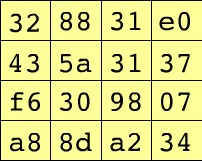
\includegraphics[width=0.7\textwidth]{./png/S002.jpg}
    \caption{Шифр Rail Fence}%
\end{figure}

\steppar{1} Создан файл с открытым текстом, содержащим последовательность цифр 12345678900987654321.

\steppar{1} Произведена зашифровка и расшифровка созданного текста. Результаты на рисунке~\label{img:fence:2}
\begin{figure}[h]
    \centering
    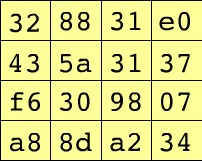
\includegraphics[width=0.7\textwidth]{./png/S002.jpg}
    \caption{Зашифровка и расшифровка}%
    \label{img:fence:2}
\end{figure}

\steppar{1} Коллеге слева сгенерирована последовательность INTERNATIONALE и зашифрована с числом строк $8$: INETLEARNNOAIT.\@

Коллега расшифровывала последовательность меньше нескольких минут путём перебора числа строк.

\steppar{1} Полученная от коллеги слева последовательность: BKLIOINVNA.\@ Ход расшифровки представлен на рис.~\ref{img:fence:1}
\begin{figure}[h]
    \centering
    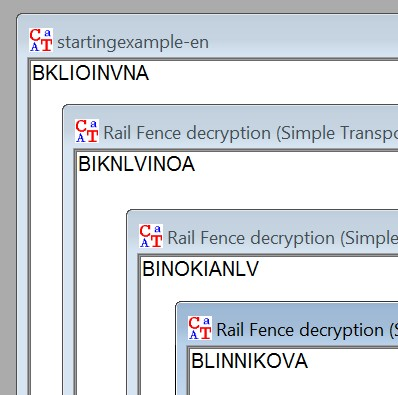
\includegraphics[width=0.7\textwidth]{./png/S001.jpg}
    \caption{Ход расшифровки последовательности}%
    \label{img:fence:1}
\end{figure}
С 4-й попытки выяснено, что последовательность зашифрована с числом строк $4$. Соответственно, это ключ. 


\section*{Выводы}

\end{document}
